\begin{figure}
    \centering
    \setlength{\tabcolsep}{1pt}
    {\small
    \begin{tabular}{cccc}
        %
        \multicolumn{4}{c}{``A red velvet chesterfield chair''} \\
        %
                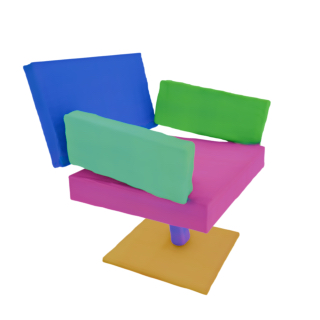
\includegraphics[width=0.24\linewidth, trim=20 20 40 40, clip]{images/editings/spice-e/velvet_chair/guidance/chair_0000.jpg} &
                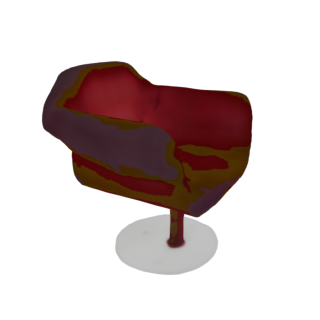
\includegraphics[width=0.24\linewidth, trim=40 40 60 60, clip]{images/editings/spice-e/velvet_chair/spice-e/shap-e_tile_0.png} &

                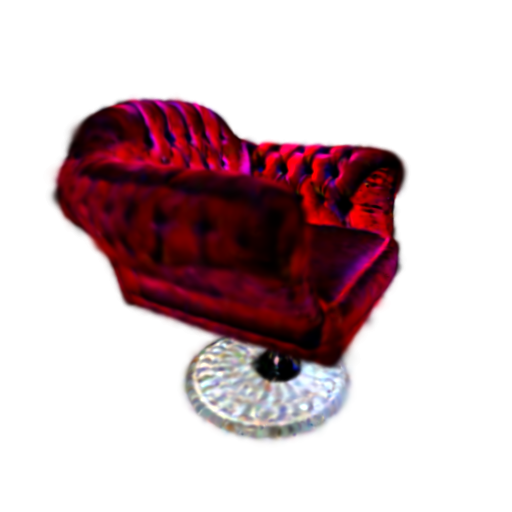
\includegraphics[width=0.24\linewidth, trim=60 60 100 90, clip]{images/editings/spice-e/velvet_chair/sds/1.png} &
                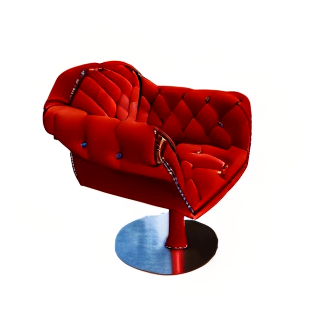
\includegraphics[width=0.24\linewidth, trim=40 40 60 60, clip]{images/editings/spice-e/velvet_chair/sharp-e/a_red_velvet_chair_2_75_steps_batch_0_a_chesterfield_light_red_velvet_chair_tile_0.png} \\
        %
                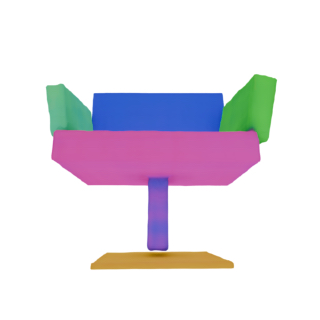
\includegraphics[width=0.24\linewidth, trim=40 50 40 60, clip]{images/editings/spice-e/velvet_chair/guidance/chair_0001.jpg} &
                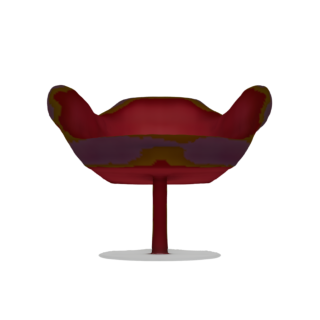
\includegraphics[width=0.24\linewidth, trim=40 50 40 60, clip]{images/editings/spice-e/velvet_chair/spice-e/shap-e_tile_1.png} &
                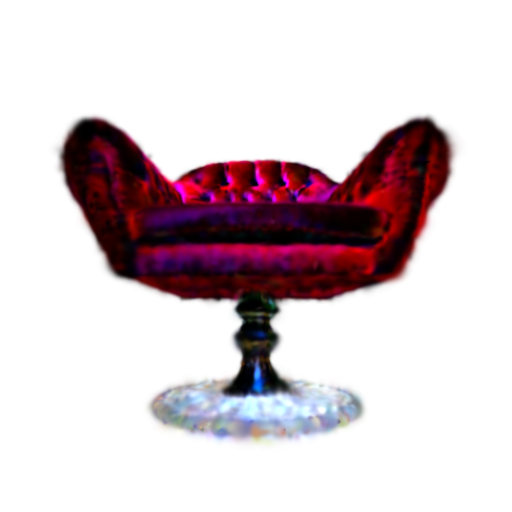
\includegraphics[width=0.24\linewidth, trim=50 60 50 90, clip]{images/editings/spice-e/velvet_chair/sds/0.png} &
                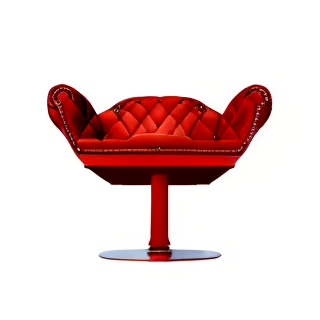
\includegraphics[width=0.24\linewidth, trim=40 50 40 60, clip]{images/editings/spice-e/velvet_chair/sharp-e/a_red_velvet_chair_2_75_steps_batch_0_a_chesterfield_light_red_velvet_chair_tile_1.png} \\
                
        %
        \multicolumn{4}{c}{``A cargo spaceship''} \\
        %
                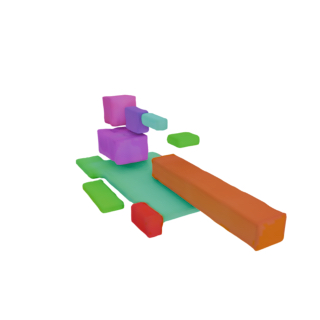
\includegraphics[width=0.24\linewidth, trim=60 60 20 50, clip]{images/editings/spice-e/space_ship/guidance/render_0002.jpg} &
                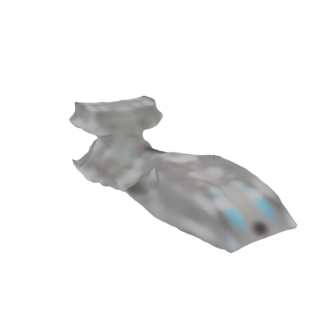
\includegraphics[width=0.24\linewidth, trim=60 60 20 50, clip]{images/editings/spice-e/space_ship/spice-e/spice-e_tile_2.png} &
                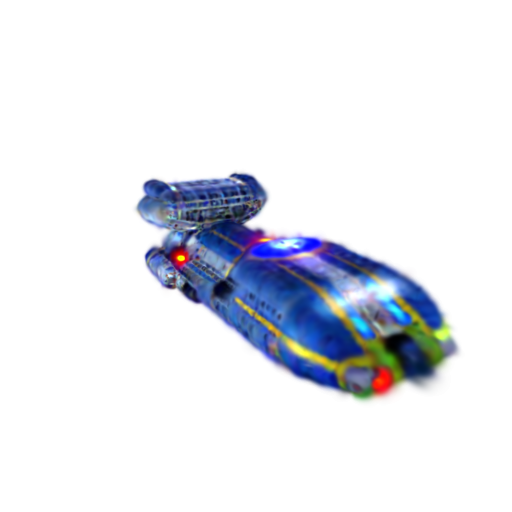
\includegraphics[width=0.24\linewidth, trim=60 60 20 105, clip]{images/editings/spice-e/space_ship/sds/2.png}  &
                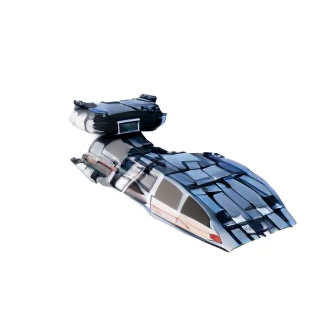
\includegraphics[width=0.24\linewidth, trim=60 60 20 50, clip]{images/editings/spice-e/space_ship/sharp_e/sharp_e_tile_2.png} \\
                
        %
                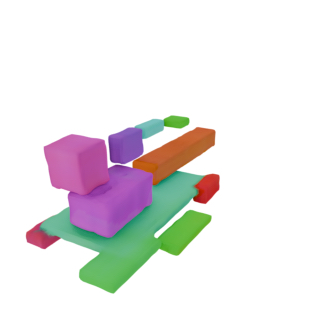
\includegraphics[width=0.24\linewidth, trim=0 0 70 70, clip]{images/editings/spice-e/space_ship/guidance/render_0000-2.jpg} &
                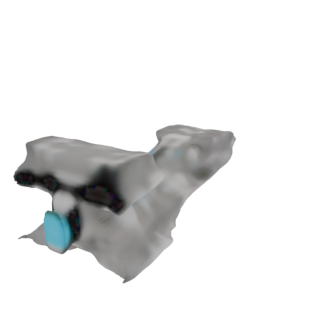
\includegraphics[width=0.24\linewidth, trim=0 0 70 70, clip]{images/editings/spice-e/space_ship/spice-e/spice-e_tile_0.png} &
                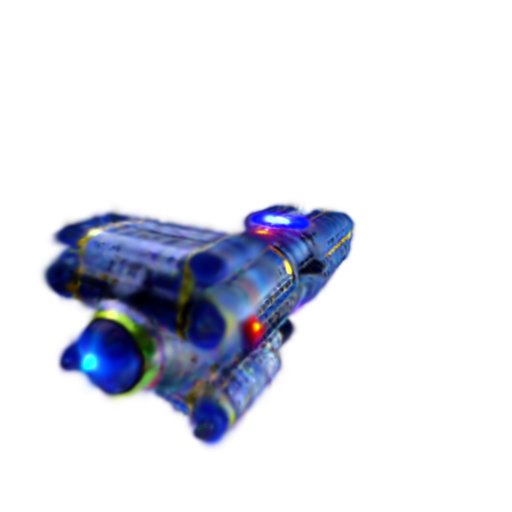
\includegraphics[width=0.24\linewidth, trim=0 0 95 95, clip]{images/editings/spice-e/space_ship/sds/0.png}&
                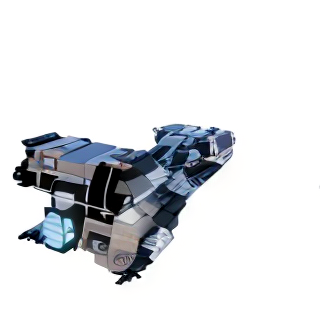
\includegraphics[width=0.24\linewidth, trim=0 0 70 70, clip]{images/editings/spice-e/space_ship/sharp_e/sharp_e_tile_0.png}  \\
                
        %
        Abstract 3D  & Spice-E & w/ SDS & w/ \ourname \\
        Guidance & & refinement & refinement
    \end{tabular}
    }
    \vspace{-8pt}
    \caption{
    \ourname{} refines outputs generated by Spice-E, in a faster and more visually appealing way than an SDS-based refinement.
    }
    \vspace{-14pt}
    \label{fig:controlled-generation}
\end{figure}